\chapter{Descripción}\label{chapter03}

AIVA es un sistema web orientado a pequeñas y medianas empresas de alimentos perecederos, como por ejemplo panaderías y confiterías, que busca reducir mermas y quiebres de stock mediante la planificación de producción y reposición basada en datos. La propuesta integra, en una única plataforma, la captura flexible de ventas (punto de venta, importación de CSV y carga asistida por imágenes), el enriquecimiento contextual (clima, calendario y patrones semanales) y un módulo de predicción de demanda diaria por producto. Sobre esta base, el sistema ofrece visualizaciones ejecutivas (backoffice), un asistente conversacional para consultas operativas y un mecanismo de alertas que anticipa situaciones de sobreproducción o faltantes. 

El núcleo analítico del sistema combina el historial transaccional con variables exógenas para estimar la demanda esperada a corto plazo. Este módulo implementa un enfoque heurístico transparente centrado en tendencia, estacionalidad y condiciones meteorológicas, con un diseño abierto a la incorporación de modelos estadísticos y de aprendizaje automático más avanzados. La arquitectura prioriza componentes de bajo costo y rápida adopción, asegurando trazabilidad de datos, reproducibilidad de resultados y una experiencia de usuario alineada con los flujos cotidianos del negocio.


\vspace{1cm}
\section{Requerimientos del sistema}
Esta sección especifica las condiciones verificables que delimitan el alcance de AIVA. Se formulan en modo imperativo (“El sistema debe …”) para facilitar su prueba y aceptación. Se organizan en dos grupos: funcionales (capacidades observables) y no funcionales (calidades y restricciones transversales).

\subsection{Requerimientos funcionales}
Definen lo que el sistema hace de cara al usuario y a los procesos de negocio (captura de datos, análisis y presentación). Recogen sólo lo esencial para operar AIVA extremo a extremo, sin imponer detalles de implementación.

\begin{enumerate}[label=RF-\arabic*., leftmargin=*, nosep]
  \item El sistema debe permitir registro, verificación de correo e inicio/cierre de sesión.
  \item El sistema debe asignar automáticamente un plan gratuito al alta y reflejarlo en la sesión.
  \item El sistema debe mantener la sesión activa y renovar credenciales mientras sean válidas.
  \item El sistema debe gestionar productos y categorías con operaciones CRUD.
  \item El sistema debe permitir cargar productos y ventas históricas vía CSV con validación previa.
  \item El sistema debe registrar ventas mediante un flujo POS con totales e ítems por producto.
  \item El sistema debe enriquecer transacciones con contexto (fecha, día, clima, feriados/fin de semana).
  \item El sistema debe generar predicciones de demanda por producto considerando tendencia, estacionalidad y clima.
  \item El sistema debe asociar a cada predicción nivel de confianza, factores explicativos y recomendación de stock.
  \item El sistema debe persistir predicciones por usuario y período y permitir su recalculo bajo demanda.
  \item El sistema debe exponer un tablero con KPIs de ventas, clima y predicciones vigentes.
  \item El sistema debe ofrecer un asistente conversacional para consultas y navegación guiada (\texttt{/api/chat}).
  \item El sistema debe generar y listar alertas operativas (stock bajo, sobreproducción potencial, feriados).
  \item El sistema debe filtrar todos los datos por el identificador del usuario autenticado.
\end{enumerate}

\subsection{Requerimientos no funcionales}
Establecen cualidades globales del sistema (seguridad, desempeño, mantenibilidad, confiabilidad). Limitan cómo se implementan los servicios, sin modificar el comportamiento funcional.

\begin{enumerate}[label=RNF-\arabic*., leftmargin=*, nosep]

  \item El sistema debe garantizar la seguridad y privacidad de la información, protegiendo todos los recursos mediante mecanismos de autenticación y autorización basados en estándares actuales. Las credenciales deberán transmitirse exclusivamente por conexiones seguras (HTTPS) y almacenarse de forma cifrada. Asimismo, se debe aplicar segmentación de datos por \texttt{user\_id} (RLS o equivalente) para asegurar que cada usuario acceda únicamente a sus propios registros.

  \item El sistema debe ofrecer un desempeño adecuado a su uso interactivo, proporcionando tiempos de respuesta inferiores a 2\,segundos durante la navegación del \textit{dashboard}, y ejecutando los procesos de predicción bajo demanda en tiempos compatibles con el uso continuo (orden de segundos). Los servicios deberán mantener una disponibilidad no inferior al 99\,\% mensual, asegurando estabilidad operativa y experiencia fluida.

  \item El sistema debe manejar errores, fallas externas y entradas inválidas de forma controlada, mostrando mensajes claros, categorizados y recuperables que permitan al usuario continuar la operación o corregir el ingreso. Además, deberá registrar todos los eventos relevantes, como errores, importaciones y cálculos, en un sistema de auditoría que permita trazabilidad y diagnóstico posterior.

  \item El sistema debe garantizar la integridad y consistencia de la base de datos, aplicando restricciones de integridad referencial y ejecutando todas las operaciones críticas de escritura mediante transacciones atómicas. En particular, las altas de ventas deberán registrarse de manera completa y coherente, evitando duplicados, pérdidas de datos o inconsistencias lógicas.

  \item El sistema debe asegurar la usabilidad y accesibilidad de la interfaz, siendo compatible con los principales navegadores modernos de escritorio y adaptándose correctamente a distintos tamaños de pantalla. Deberá cumplir las pautas básicas de accesibilidad web, incluyendo contraste de color adecuado y navegación por teclado en los controles principales, priorizando la claridad visual y la facilidad de uso para cualquier usuario.

  \item El sistema debe mantener altos estándares de mantenibilidad y calidad del código, organizando su arquitectura en módulos tipados y reutilizables, con convenciones de estilo consistentes y documentación técnica actualizada. Los secretos y claves de acceso deberán gestionarse mediante variables de entorno, con rotación periódica de credenciales. Además, se deben realizar respaldos automáticos de los datos críticos y versionar todas las migraciones de base de datos y despliegues, garantizando trazabilidad y control de versiones en todo el ciclo de vida del sistema.

\end{enumerate}

\section{Análisis FODA}\label{sec:foda}

El análisis FODA (acrónimo de Fortalezas, Oportunidades, Debilidades y Amenazas) constituye una herramienta metodológica ampliamente utilizada en la gestión estratégica de proyectos y organizaciones. Su finalidad es evaluar de manera integral los factores internos y externos que inciden en el desempeño de un sistema, identificando los aspectos positivos y negativos que pueden influir en su desarrollo. A partir de esta evaluación, es posible definir estrategias orientadas a potenciar las fortalezas, aprovechar las oportunidades, minimizar las debilidades y anticipar las amenazas, contribuyendo así a la toma de decisiones fundamentadas y sostenibles.

El objetivo del presente análisis es examinar la posición estratégica del sistema AIVA dentro del entorno tecnológico, económico y social en el que se inserta. AIVA es una plataforma de inteligencia artificial aplicada a la predicción de demanda en comercios de productos perecederos. En este contexto, el análisis FODA permite determinar las ventajas competitivas del proyecto, las limitaciones que podrían afectar su implementación, las oportunidades de crecimiento que ofrece el mercado y los riesgos asociados al entorno externo, con el propósito de establecer una visión clara y sustentada sobre su viabilidad y potencial de escalabilidad.

\subsection{Análisis interno}

En el análisis interno se identifican las principales fortalezas y debilidades del proyecto. 

Entre las fortalezas más relevantes, se destaca la propuesta tecnológica integral de AIVA, que combina predicción de demanda mediante algoritmos de inteligencia artificial, un asistente conversacional basado en lenguaje natural y carga automatizada de registros mediante tecnologías OCR y modelos de lenguaje extensos (LLMs). Esta integración de herramientas convierte al sistema en una solución innovadora y de alto valor agregado para pequeños comercios. Asimismo, su diseño centrado en la usabilidad y accesibilidad favorece la adopción por parte de usuarios sin conocimientos técnicos, a diferencia de las soluciones corporativas que demandan infraestructura avanzada. 

Otro aspecto sobresaliente es la adaptación del modelo al contexto local, incorporando variables como condiciones climáticas, feriados y patrones de consumo característicos del Área Metropolitana de Buenos Aires, lo que incrementa la precisión de las predicciones. Desde el punto de vista estratégico, AIVA contribuye al \textit{Objetivo de Desarrollo Sostenible N.º 12 (Producción y Consumo Responsables)} al promover la reducción del desperdicio alimentario y el uso eficiente de recursos. Además, su modelo de negocio, basado en un esquema de suscripción mensual con período de prueba gratuito (free trial), presenta indicadores financieros favorables, con un valor actual neto positivo, una tasa interna de retorno superior al 50\,\% y un período de recupero estimado en aproximadamente dos años. Finalmente, la arquitectura moderna y modular del sistema, basada en tecnologías como Next.js, Supabase y OpenWeather API, asegura un funcionamiento eficiente, escalable y de mantenimiento simple.

Entre las debilidades, se identifica la dependencia de la calidad y cantidad de los datos iniciales que los usuarios carguen en el sistema, dado que la precisión de los modelos predictivos se encuentra directamente relacionada con la disponibilidad y consistencia de dichos registros. Asimismo, la continuidad del proyecto requiere inversión constante y recursos técnicos especializados para el mantenimiento y actualización de los modelos de inteligencia artificial, lo cual puede representar una limitación en etapas tempranas de expansión. Otro desafío relevante es la curva de adopción tecnológica: algunos usuarios, especialmente en comercios tradicionales, pueden mostrar resistencia o dificultades al incorporar nuevas herramientas digitales, lo que exige estrategias de acompañamiento y capacitación. Finalmente, la dependencia de proveedores externos como OpenAI o Supabase introduce vulnerabilidades ante posibles variaciones en costos, políticas de uso o disponibilidad de servicios.

\subsection{Análisis externo}

El análisis externo considera los factores del entorno que pueden influir en el desempeño del proyecto, tanto de manera positiva como negativa. 

En cuanto a las oportunidades, se observa un contexto favorable caracterizado por una creciente demanda de digitalización en pequeñas y medianas empresas, muchas de las cuales carecen de herramientas de análisis avanzadas. Este panorama abre un amplio espacio de inserción para soluciones accesibles como AIVA, que facilitan la transición hacia la gestión inteligente de datos. Además, la expansión global del mercado de inteligencia artificial aplicada al sector minorista y alimentario impulsa la adopción de tecnologías predictivas orientadas a la optimización de la producción y la reducción de mermas. 

Las entrevistas y encuestas realizadas a comerciantes confirman una necesidad real y validada de herramientas que mejoren la planificación operativa, lo que respalda la pertinencia del sistema. También se identifican oportunidades de crecimiento mediante alianzas estratégicas con cámaras empresariales, asociaciones gastronómicas o programas de innovación tecnológica, que podrían acelerar la adopción y fortalecer el posicionamiento de la plataforma. Finalmente, la naturaleza SaaS (Software as a Service) y la arquitectura modular de AIVA permiten su adaptación a otros mercados de América Latina con ajustes mínimos, potenciando su escalabilidad regional.

Entre las amenazas más relevantes, se encuentra la competencia de soluciones internacionales consolidadas, como las ofrecidas por SAP, Oracle o Blue Yonder, que cuentan con una mayor trayectoria y recursos, aunque orientadas a grandes corporaciones y con costos elevados. No obstante, su presencia podría limitar la participación de nuevos actores en determinados segmentos del mercado. La inestabilidad macroeconómica argentina representa otro factor de riesgo, ya que la inflación, las variaciones del tipo de cambio y las restricciones financieras pueden afectar la rentabilidad y el acceso a recursos tecnológicos. 

Asimismo, la baja digitalización estructural de muchos comercios minoristas constituye una barrera para la adopción inicial del sistema, especialmente en regiones con infraestructura tecnológica limitada. El rápido ritmo de evolución en los modelos de inteligencia artificial exige actualizaciones constantes para mantener la competitividad y vigencia del producto. Finalmente, los riesgos asociados a la ciberseguridad y la protección de datos requieren políticas estrictas de confidencialidad y cumplimiento normativo, dada la sensibilidad de la información comercial que el sistema maneja.

\subsection{Síntesis del análisis}

En síntesis, el análisis FODA evidencia que AIVA presenta una posición estratégica favorable dentro del contexto local, sustentada en su carácter innovador, su enfoque sostenible y su adaptabilidad a las necesidades de las PYMEs argentinas. Las fortalezas y oportunidades identificadas superan ampliamente las debilidades y amenazas, consolidando al proyecto como una solución viable, escalable y con impacto positivo tanto económico como ambiental. Este diagnóstico permite concluir que AIVA posee una base sólida para su implementación, expansión y sostenimiento en el tiempo, contribuyendo al desarrollo tecnológico y a la eficiencia operativa del sector de productos perecederos.


\vspace{1cm}
\section{Historias de usuario}
Esta sección captura, en lenguaje natural, necesidades y objetivos de los actores del sistema. Cada historia sigue el formato \emph{«Como [rol], quiero [objetivo] para [beneficio]»} e incluye criterios de aceptación sintéticos.

\begin{enumerate}[label=HU-\arabic*., leftmargin=*, nosep]

\item Como \textbf{Comerciante nuevo}, quiero registrarme e iniciar sesión con verificación de correo para comenzar a usar AIVA de forma segura.
\begin{itemize}[nosep]
\item No se permite acceso hasta confirmar el correo; al confirmar, queda sesión activa.
\item Tras el alta, se asigna automáticamente el plan gratuito y se refleja en la sesión.
\end{itemize}

\item Como \textbf{Comerciante}, quiero fijar mi ubicación por defecto para que el sistema incorpore clima local en análisis y predicciones.
\begin{itemize}[nosep]
\item La ubicación se persiste y es editable por el usuario.
\item Las consultas al servicio de clima usan la ubicación guardada.
\end{itemize}

\item Como \textbf{Administrador de catálogo}, quiero gestionar productos y categorías (crear/editar/eliminar) para mantener actualizado el inventario.
\begin{itemize}[nosep]
\item Validación de campos obligatorios y unicidad por usuario.
\item Historial de movimientos de stock visible por producto.
\end{itemize}

\item Como \textbf{Administrador de catálogo}, quiero cargar productos por CSV con vista previa para acelerar altas masivas sin errores.
\begin{itemize}[nosep]
\item Se validan columnas mínimas; se muestra resumen de aceptadas/rechazadas.
\item La importación es idempotente y permite revertir en caso de error.
\end{itemize}

\item Como \textbf{Cajero/a}, quiero registrar una venta tipo POS con carrito y totales para asentar transacciones rápidamente.
\begin{itemize}[nosep]
\item La confirmación crea venta e ítems de forma atómica y actualiza stock.
\item La transacción queda enriquecida con fecha/día y banderas de contexto.
\end{itemize}

\item Como \textbf{Analista}, quiero importar ventas históricas (CSV) para consolidar el histórico que alimenta reportes y predicciones.
\begin{itemize}[nosep]
\item Normalización de fechas/productos y registro descargable de errores.
\item Detección de duplicados para evitar dobles cargas (idempotencia).
\end{itemize}

\item Como \textbf{Operador}, quiero registrar ventas asistidas por imágenes (OCR) para acelerar la carga desde comprobantes.
\begin{itemize}[nosep]
\item Estados visibles: en cola, procesando, listo; notificación al completar.
\item Edición/corrección antes de confirmar el alta definitiva.
\end{itemize}

\item Como \textbf{Responsable de producción}, quiero ver y recalcular predicciones (hoy/semana/mes) para planificar elaboración y reposición.
\begin{itemize}[nosep]
\item Cada predicción incluye confianza, factores y recomendación de stock.
\item Se persisten por fecha/usuario y se marcan como vigentes.
\end{itemize}

\item Como \textbf{Encargado}, quiero recibir alertas de quiebre/sobreproducción y feriados para actuar preventivamente.
\begin{itemize}[nosep]
\item Listado priorizado por criticidad con fecha y producto.
\item Enlaces a la acción sugerida (ajuste de producción/stock).
\end{itemize}

\item Como \textbf{Gerente}, quiero un \textit{dashboard} y reportes por período, producto y categoría para monitorear desempeño y tendencias.
\begin{itemize}[nosep]
\item Gráficos comparan observado vs.\ predicho con filtros persistentes.
\item Exportes básicos (tabla/gráfico) para análisis externo.
\end{itemize}

\item Como \textbf{Usuario}, quiero consultar al asistente conversacional para obtener métricas y ejecutar tareas frecuentes sin salir del flujo.
\begin{itemize}[nosep]
\item Gestión de conversaciones (crear/cambiar/archivar) y copia de respuestas.
\item Manejo de errores categorizado y posibilidad de cancelar la respuesta.
\end{itemize}

\item Como \textbf{Usuario de plan gratuito}, quiero poder adquirir una suscripción desde la app para habilitar capacidades avanzadas.
\begin{itemize}[nosep]
\item Verificación de identidad y confirmación de pago cuando corresponda.
\item La nueva capacidad se refleja de inmediato en la sesión.
\end{itemize}

\end{enumerate}


\vspace{1cm}
\section{Interfaz gráfica}
En esta sección se expone la interfaz gráfica desarrollada para la interacción cotidiana de los usuarios de AIVA en el entorno de comercio minorista de alimentos perecederos. La UI prioriza baja fricción operativa, consistencia visual y señales claras para la toma de decisiones, con patrones reutilizables que reducen la curva de aprendizaje. A continuación se describen las dos pantallas más relevantes por su impacto en el trabajo diario: el asistente conversacional (chatbot) y el módulo de predicción de demanda.

\subsection{Asistente conversacional (chatbot)}
\begin{figure}[!htbp]
  \centering
  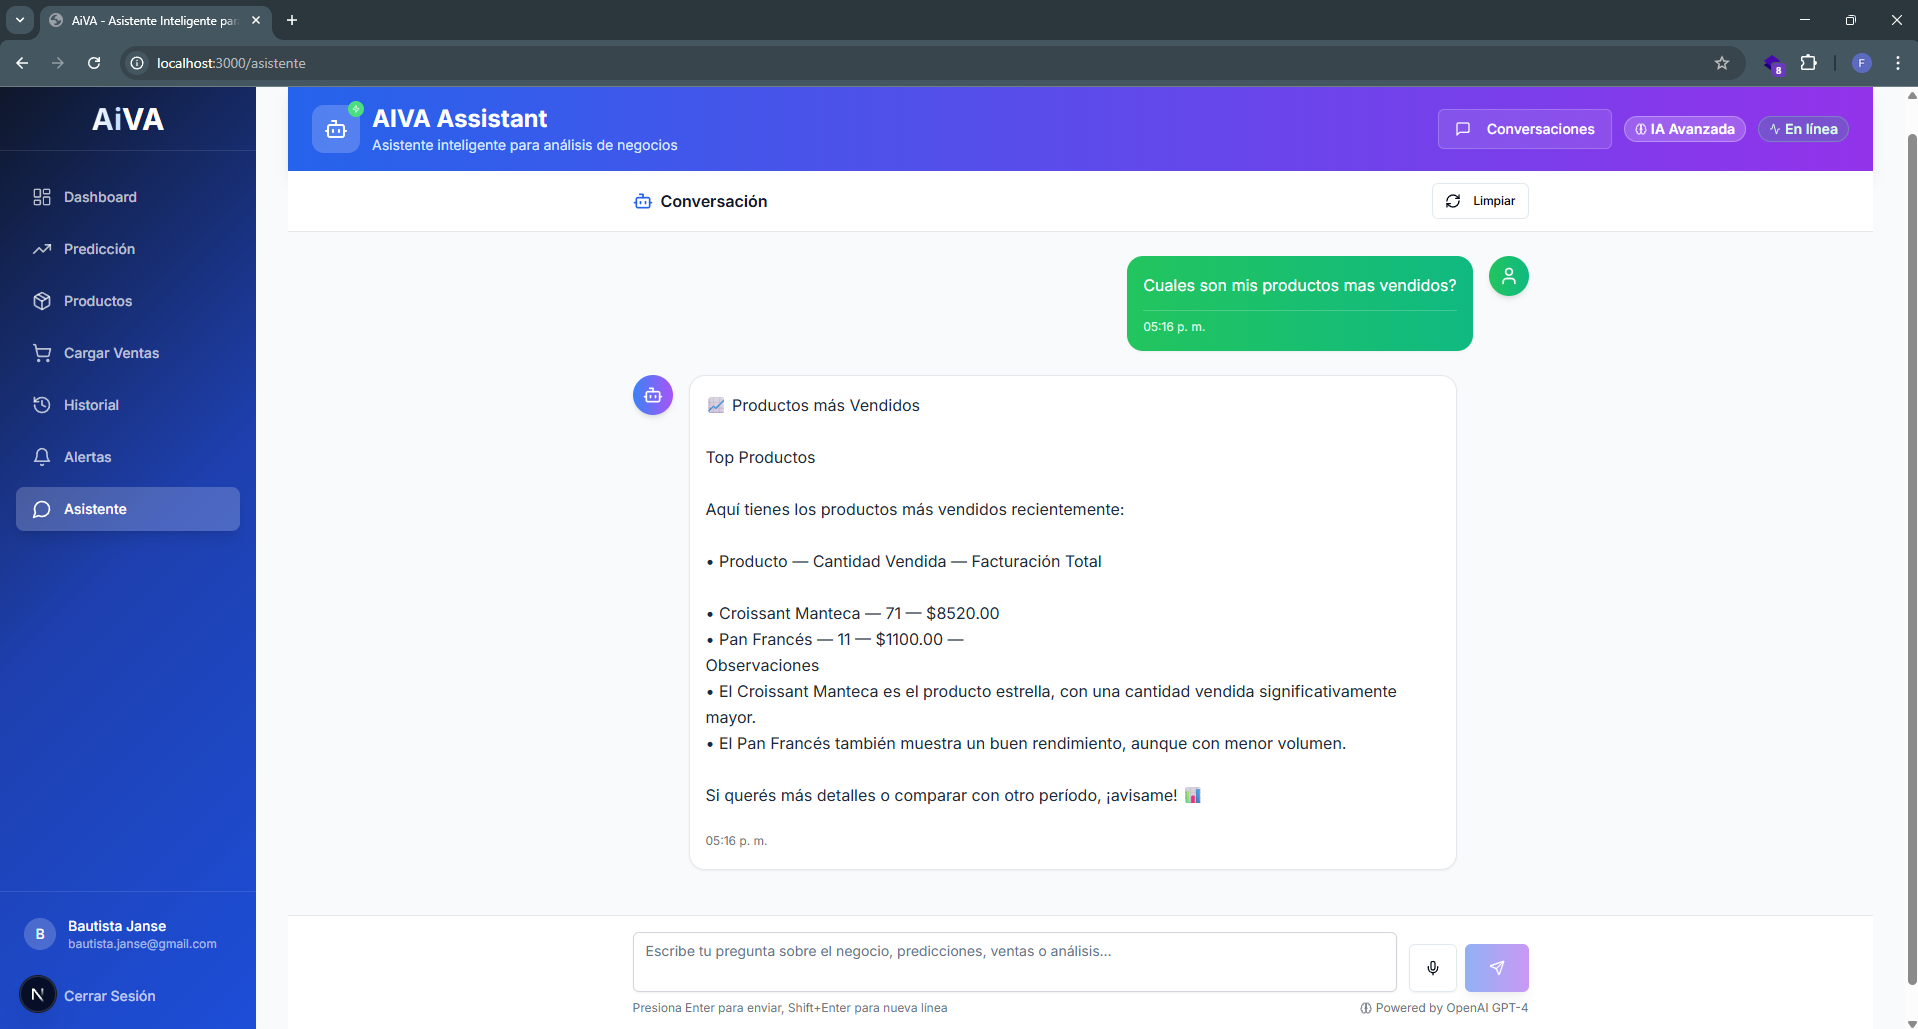
\includegraphics[width=0.92\textwidth]{images/chatbotPage.png}
  \caption{Asistente conversacional (chatbot) -- Fuente: elaboración propia}
  \label{fig:ui-chatbot}
\end{figure}
La pantalla del asistente provee un canal de interacción en lenguaje natural para consultar métricas, navegar a vistas operativas y disparar acciones frecuentes sin abandonar el flujo de trabajo. El encabezado, con gradiente azul–violeta, muestra el estado del servicio mediante la insignia («En línea») y un selector de conversaciones que permite crear, cambiar y archivar hilos, favoreciendo la continuidad y la trazabilidad de consultas.

El área central es un historial desplazable con burbujas alineadas según el rol: los mensajes del usuario se muestran a la derecha y las respuestas del asistente, a la izquierda. Cada mensaje incorpora marca de tiempo y, en el caso del asistente, una acción para copiar el contenido. Cuando no hay historial, se presenta un saludo dinámico según la hora y atajos de acción (“Ver predicciones de mañana”, “Analizar ventas de esta semana”) que precargan consultas típicas para reducir fricción.

La barra inferior concentra la entrada de texto, con envío por Enter y salto de línea con \textit{Shift+Enter}, y botones para enviar o limpiar la conversación. Durante el procesamiento se indica actividad y se habilita la interrupción segura de la respuesta. La comunicación con el backend se realiza autenticada (token de sesión de Supabase) contra el endpoint interno \texttt{/api/chat}; se contemplan estados de error categorizados (cuota, servicio, autenticación, cancelación y red) con retroalimentación visual y mensajes recuperables. En conjunto, el diseño prioriza velocidad de uso, consistencia con el resto de la interfaz y control explícito sobre el ciclo de la conversación.

\subsection{Procesamiento de la consulta}
Cuando el usuario ingresa una consulta en el chat, el asistente procesa el mensaje y determina la intención de la pregunta a partir del lenguaje natural. En lugar de devolver una respuesta predefinida o aproximada, el agente genera de manera dinámica una consulta SQL parametrizada que traduce esa necesidad en una instrucción concreta sobre la base de datos. Esta consulta, siempre restringida a operaciones de solo lectura y filtrada por el identificador del usuario, se ejecuta en Supabase sobre el motor Postgres, garantizando seguridad y acceso únicamente a la información correspondiente. Una vez obtenidos los resultados, el asistente procesa los datos para calcular métricas, agrupar valores y elaborar indicadores relevantes, que luego son redactados en un formato comprensible y ejecutivo. De esta manera, el usuario recibe una respuesta clara y contextualizada, sustentada en datos reales y actualizados, sin exposición de detalles técnicos. El enfoque adoptado constituye el núcleo innovador de la solución: transformar de forma automática las consultas en lenguaje natural en consultas SQL seguras, ejecutarlas en tiempo real y presentar los resultados de manera amigable dentro del flujo conversacional.

\subsection{Predicción de demanda}
\begin{figure}[!htbp]
\centering
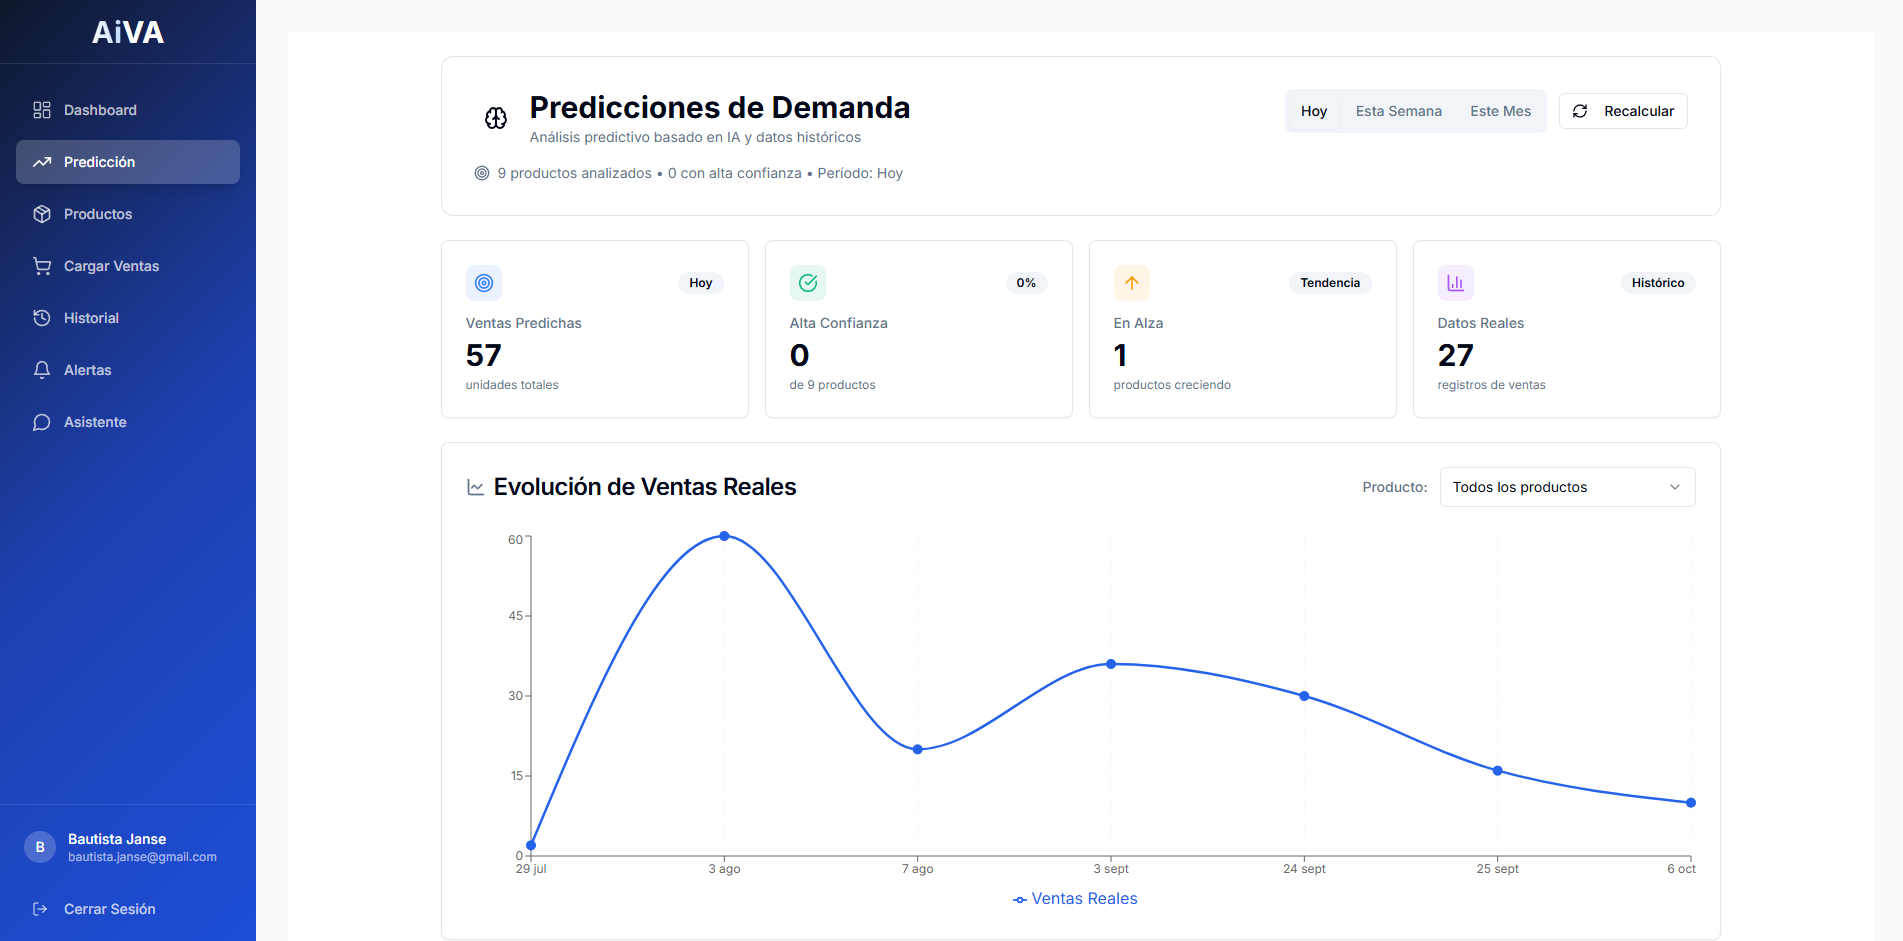
\includegraphics[width=0.95\textwidth]{images/prediccionPage.png}
\caption{Predicción de demanda -- Fuente: elaboración propia}
\label{fig:ui-prediccion}
\end{figure}
La pantalla de predicción concentra el cálculo y la consulta de estimaciones por producto. El encabezado permite elegir el período de análisis (hoy, semana, mes) y recalcular bajo demanda; al mismo tiempo, resume el estado del proceso con indicadores clave (ventas predichas, confianza alta, tendencia positiva y volumen de datos históricos). La sección analítica combina un gráfico de ventas reales filtrable por producto con tres vistas complementarias: un resumen ejecutivo (top productos y riesgos), un detalle tabular con filtros por producto/categoría y umbral de confianza, y un historial de ventas con contexto (clima, fin de semana, feriados). Las predicciones se generan en tiempo real mediante el servicio de predicción y se persisten en la base (tabla \texttt{predictions}, por usuario y período), priorizando trazabilidad, consistencia visual con el dashboard y manejo explícito de errores/estados para decisiones operativas rápidas.

\subsection{Procesamiento de prediccón}
Cuando se registra una venta en el sistema, además de almacenar la transacción, se capturan variables contextuales relevantes como fecha y hora, condiciones climáticas, feriados y características del producto (por ejemplo, si es perecedero). Estos datos se combinan con el historial reciente de ventas para estimar la demanda futura de cada producto, aplicando factores de tendencia, estacionalidad y contexto temporal. El resultado de este proceso es una predicción por período (hoy, semana o mes) que incluye métricas de cantidad esperada, nivel de confianza, tendencia y recomendaciones de stock. Las predicciones generadas se guardan automáticamente en la base de datos en la tabla \texttt{predictions}, asociadas al usuario y al período, lo que asegura que luego puedan ser consultadas en tiempo real desde la interfaz conversacional o visualizadas en la pantalla analítica. De este modo, cada nueva venta no solo actualiza el registro histórico, sino que alimenta y refina las estimaciones disponibles para la toma de decisiones.


\section{Tecnologías utilizadas}\label{sec:tecnologias}
A continuación se detallan las tecnologías empleadas en AIVA, explicando su rol dentro de la solución, el modo de integración y los criterios que justifican su elección. La selección prioriza un balance entre rapidez de implementación, bajo costo operativo, mantenibilidad y adecuación a los requerimientos del sistema.

\subsection{Next.js (React + TypeScript)}
Next.js es un \textit{framework} sobre React que incorpora enrutamiento, optimizaciones de rendimiento y opciones de renderizado (cliente/servidor). En AIVA se utiliza para:
\begin{itemize}
    \item Implementar la interfaz web con componentes reutilizables y tipado estático (TypeScript), reduciendo defectos en tiempo de compilación.
    \item Organizar el ruteo (App Router) separando vistas operativas (\textit{dashboard}, POS, predicción, reportes) de páginas auxiliares (autenticación, perfil).
    \item Favorecer una arquitectura mantenible (módulos, \textit{hooks} y servicios) con buena escalabilidad del frontend.
\end{itemize}
\noindent\textbf{Motivación.} Ecosistema maduro y documentación extensa, compatible con librerías modernas de UI.

\subsection{Tailwind CSS y \textit{shadcn/ui}}
Tailwind CSS provee utilidades de estilo de bajo nivel; \textit{shadcn/ui} aporta componentes accesibles basados en Tailwind.
\begin{itemize}
    \item Permiten maquetar formularios, tablas, modales y gráficos con consistencia visual y tiempos de desarrollo acotados.
    \item Estandarizan patrones de interacción (validaciones, estados de carga y error) y facilitan la personalización fina del diseño.
\end{itemize}
\noindent\textbf{Motivación.} Coherencia visual y productividad. 

\subsection{Recharts}
Recharts es una biblioteca de gráficos para React.
\begin{itemize}
    \item Se utiliza en el \textit{dashboard} y reportes para visualizar KPIs (ventas por período, productos destacados) y comparativas (predicción vs.\ observado).
    \item Ofrece componentes responsivos y composables, adecuados para vistas con filtros interactivos.
\end{itemize}
\noindent\textbf{Motivación.} Integración directa con React y bajo costo de aprendizaje.

\subsection{Supabase Auth}
Servicio gestionado para registro, inicio de sesión y manejo de sesiones (incluida verificación por correo).
\begin{itemize}
    \item Centraliza la identidad del usuario y emite \textit{tokens} para acceder a recursos protegidos.
    \item Simplifica la implementación de rutas seguras y del \textit{feature gating} por plan/suscripción.
\end{itemize}
\noindent\textbf{Motivación.} Reduce superficie de error y esfuerzo de mantenimiento respecto de una solución propia.

\subsection{PostgreSQL (vía Supabase)}
Base de datos relacional donde reside el modelo de datos.
\begin{itemize}
    \item Tablas operativas: \texttt{products}, \texttt{categories}, \texttt{sales}/\texttt{sale\_items}, \texttt{stock\_movements}.
    \item Datos analíticos y de contexto: \texttt{demand\_analysis\_data}, \texttt{predictions}/\texttt{stored\_predictions}, \texttt{weather\_data}, \texttt{plans}, \texttt{user\_subscriptions}.
    \item Soporte de integridad referencial, vistas e \textit{indexes} para consultas eficientes.
\end{itemize}
\noindent\textbf{Motivación.} Robustez y expresividad SQL para analítica operativa.

\subsection{PostgREST (Supabase)}
Capa que expone el esquema de PostgreSQL como API REST tipada.
\begin{itemize}
    \item La capa de servicios del frontend consume esta API para operaciones CRUD y consultas filtradas.
    \item Mantiene trazabilidad entre el modelo lógico y los endpoints, reduciendo código \textit{boilerplate}.
\end{itemize}
\noindent\textbf{Motivación.} Acelera la construcción de la capa de datos manteniendo convenciones REST.

\subsection{OpenWeatherMap API}
Fuente externa de variables meteorológicas usadas como factores exógenos.
\begin{itemize}
    \item Proporciona temperatura, estado del tiempo y otros atributos que se asocian a ventas y se persisten para análisis.
    \item Se contemplan \textit{fallbacks} ante indisponibilidad o latencia elevada.
\end{itemize}
\noindent\textbf{Motivación.} Cobertura suficiente para el ámbito del proyecto.

\subsection{Node.js y npm}
Entorno de ejecución y gestor de dependencias del proyecto.
\begin{itemize}
    \item Se emplea para el servidor de desarrollo, construcción del frontend y automatización de tareas (scripts).
    \item Estandariza \textit{linting}, empaquetado y gestión de versiones.
\end{itemize}
\noindent\textbf{Motivación.} \textit{Tooling} ampliamente adoptado en el ecosistema web.

\subsection{Utilitarios de CSV}
Conjunto de utilidades para ingesta histórica.
\begin{itemize}
    \item Validan formato, normalizan columnas y registran errores durante la carga de productos y ventas.
    \item Priorizan trazabilidad (filas aceptadas, rechazadas o corregidas) para reproducibilidad.
\end{itemize}
\noindent\textbf{Motivación.} Simplicidad y compatibilidad con exportaciones comunes.

\subsection{Buenas prácticas de configuración y seguridad}
\begin{itemize}
    \item Gestión de credenciales mediante variables de entorno (\texttt{.env}), evitando su versionado.
    \item Separación de entornos (desarrollo/producción) y rotación periódica de claves.
    \item En despliegues gestionados, aplicación de RLS por \textit{user\_id} para segmentación de datos.
\end{itemize}




\section{Arquitectura del sistema}

La arquitectura adoptada se basa en un modelo de tres capas 
(presentación, lógica de negocio y persistencia), apoyada en 
servicios gestionados para simplificar la operación y garantizar 
escalabilidad. El diseño busca un equilibrio entre simplicidad 
en el desarrollo y robustez en la operación, integrando 
componentes internos con servicios externos especializados.

\subsection{Capa de presentación (Front-end)}

La interfaz de usuario está implementada en \textbf{Next.js}, que cumple un doble rol:
\begin{itemize}
    \item Renderizado del front-end (formularios, dashboards, carga de datos).
    \item Exposición de endpoints internos (/api) que conectan directamente con los servicios del backend.
\end{itemize}

Los usuarios interactúan con el sistema a través de esta capa 
para gestionar productos, registrar ventas, consultar predicciones 
y atender alertas. Todas las solicitudes son enviadas al backend 
con los \textit{tokens JWT} emitidos por el servicio de autenticación.

\subsection{Capa de lógica de negocio (Backend + API Services)}

El backend, desarrollado en \textbf{Node.js}, centraliza la lógica de negocio. 
Está organizado en servicios que exponen distintos endpoints específicos.

El backend también se encarga de la validación de datos, el control 
de acceso mediante los JWT emitidos por Supabase Auth, y la interacción 
con la base de datos.

\subsection{Capa de datos (Supabase)}

La persistencia está gestionada por \textbf{Supabase}, que provee:
\begin{itemize}
    \item Base de datos PostgreSQL para almacenar usuarios, productos, ventas, predicciones y alertas.
    \item Módulo de autenticación (\textit{Supabase Auth}), encargado de la provisión y validación de tokens JWT, con \textit{Row Level Security (RLS)} configurado para restringir el acceso por \texttt{user\_id}.
\end{itemize}

La comunicación entre backend y Supabase se realiza a través de 
consultas SQL, garantizando consistencia y trazabilidad de los datos.

\subsection{Integraciones externas}

El sistema se enriquece con dos servicios externos:
\begin{itemize}
    \item \textbf{OpenWeather}: fuente de datos meteorológicos (temperatura, precipitaciones, condiciones climáticas) que son integrados al proceso de predicción de la demanda.
    \item \textbf{OpenAI}: utilizado tanto para el asistente conversacional como para procesos de OCR avanzado, ampliando la capacidad de interacción y automatización del sistema.
\end{itemize}


\begin{figure}[!htbp]
  \centering
  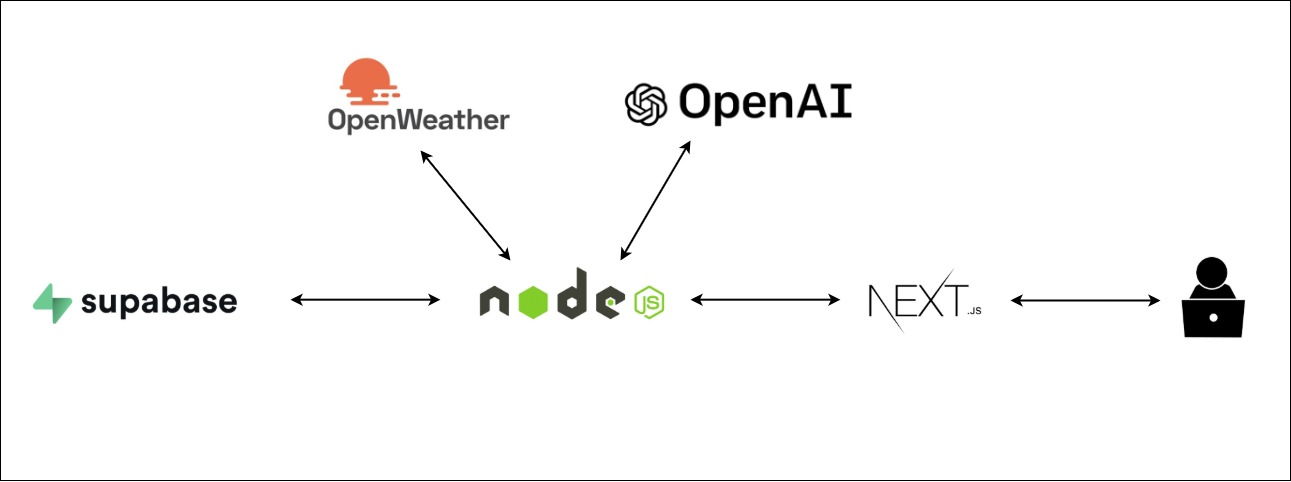
\includegraphics[width=0.92\textwidth]{images/arquitecturaAIVA.png} % <-- reemplazar por tu archivo
  \caption{Arquitectura -- Fuente :elaboración propia. Los logotipos pertenecen a sus respectivas marcas.}
  \label{fig:arquitectura-aiva}
\end{figure}
\vspace{1cm}

\section{Modelo de datos}

El diseño de la base de datos de AIVA se implementó sobre \textit{PostgreSQL} en \textit{Supabase}, priorizando la normalización, la trazabilidad y la segmentación de datos por \texttt{user\_id} para garantizar seguridad y consistencia.

El esquema integra distintas entidades relacionadas con el ciclo de ventas y predicción:

\begin{itemize}
    \item \textbf{Usuarios y perfiles}: gestionados por el módulo de autenticación de \textit{Supabase} (\texttt{auth.users}), con tabla complementaria \texttt{profiles} que almacena información adicional de cada comerciante.
    \item \textbf{Productos y categorías}: las tablas \texttt{products} y \texttt{categories} permiten organizar el catálogo con atributos como precio de costo, precio de venta, stock mínimo/máximo, vida útil y clasificación perecedera.
    \item \textbf{Ventas y detalle de ítems}: la tabla \texttt{sales} centraliza las transacciones y se relaciona con \texttt{sale\_items}, donde se registran los productos vendidos, cantidades, importes y descuentos aplicados.
    \item \textbf{Movimientos de stock}: la tabla \texttt{stock\_movements} conserva un historial de entradas y salidas, asegurando trazabilidad de inventario.
    \item \textbf{Suscripciones y planes}: las tablas \texttt{plans} y \texttt{user\_subscriptions} definen la modalidad de uso (plan gratuito o pago), el período de facturación y los límites asociados a cada cuenta.
    \item \textbf{Eventos y contexto}: la tabla \texttt{holidays\_events} registra feriados y factores de impacto; \texttt{weather\_data} almacena condiciones meteorológicas (temperatura, humedad, precipitación, viento). Estos datos enriquecen el análisis predictivo.
    \item \textbf{Análisis de demanda}: la tabla \texttt{demand\_analysis\_data} integra variables transaccionales y contextuales (día, clima, feriados, estacionalidad) para generar indicadores de tendencia, nivel de confianza y recomendaciones de stock.
\end{itemize}

En conjunto, este modelo de datos respalda la lógica analítica de AIVA, permitiendo registrar operaciones diarias, incorporar factores externos y producir predicciones personalizadas. Su organización modular facilita la escalabilidad y asegura que cada nueva transacción refuerce la capacidad predictiva del sistema.

\begin{figure}[!htbp]
  \centering
  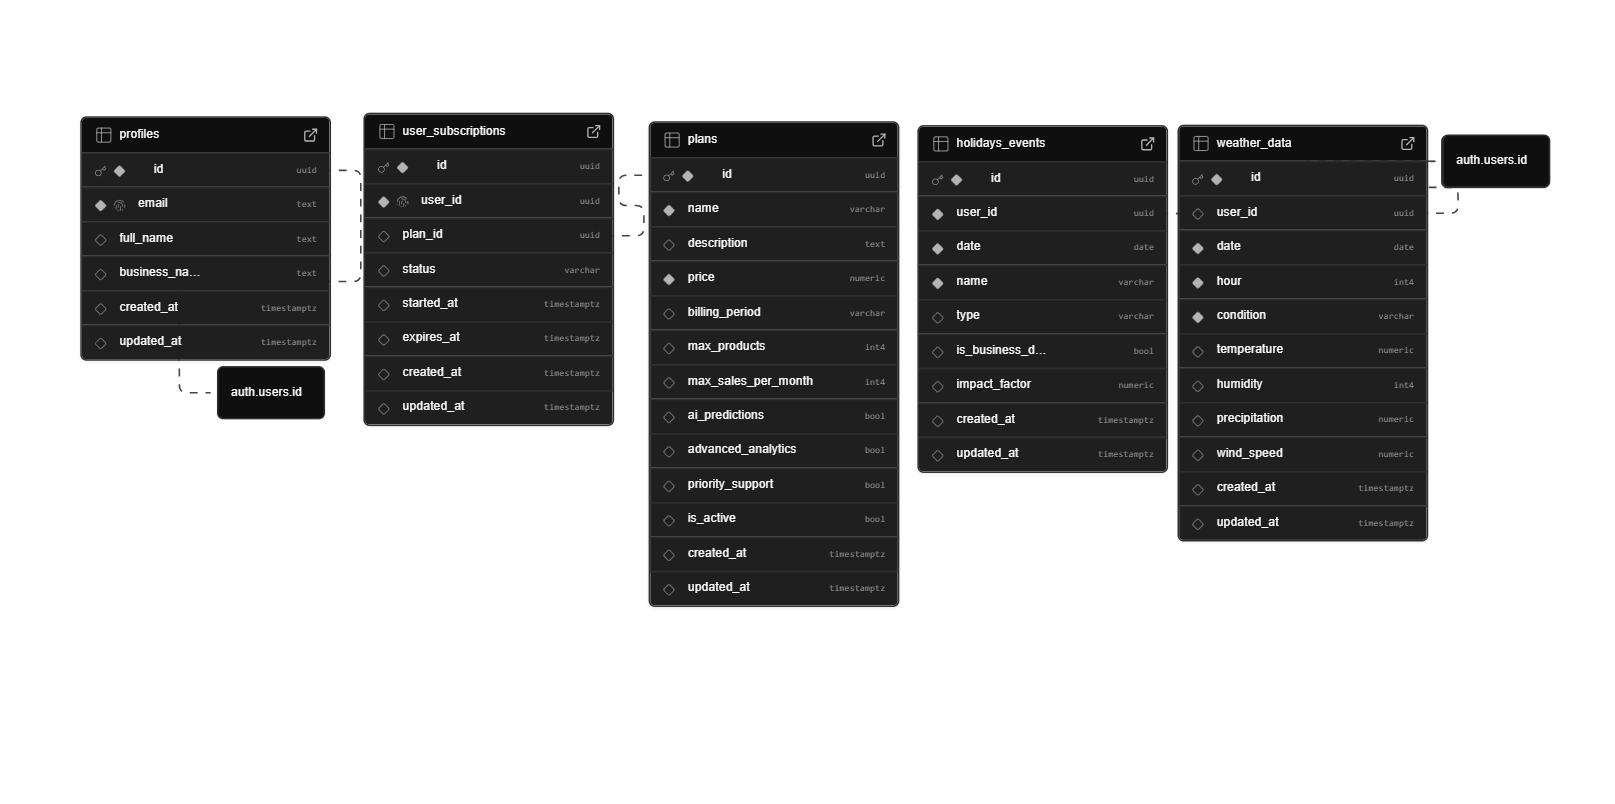
\includegraphics[width=0.95\textwidth]{images/ArquitecturaDB1.png} % <-- reemplazar por tu archivo
  \caption{Modelo de datos de AIVA 1-- Fuente: elaboración propia.}
  \label{fig:arquitectura-db}
\end{figure}
\vspace{1cm}

\begin{figure}[!htbp]
    \centering
    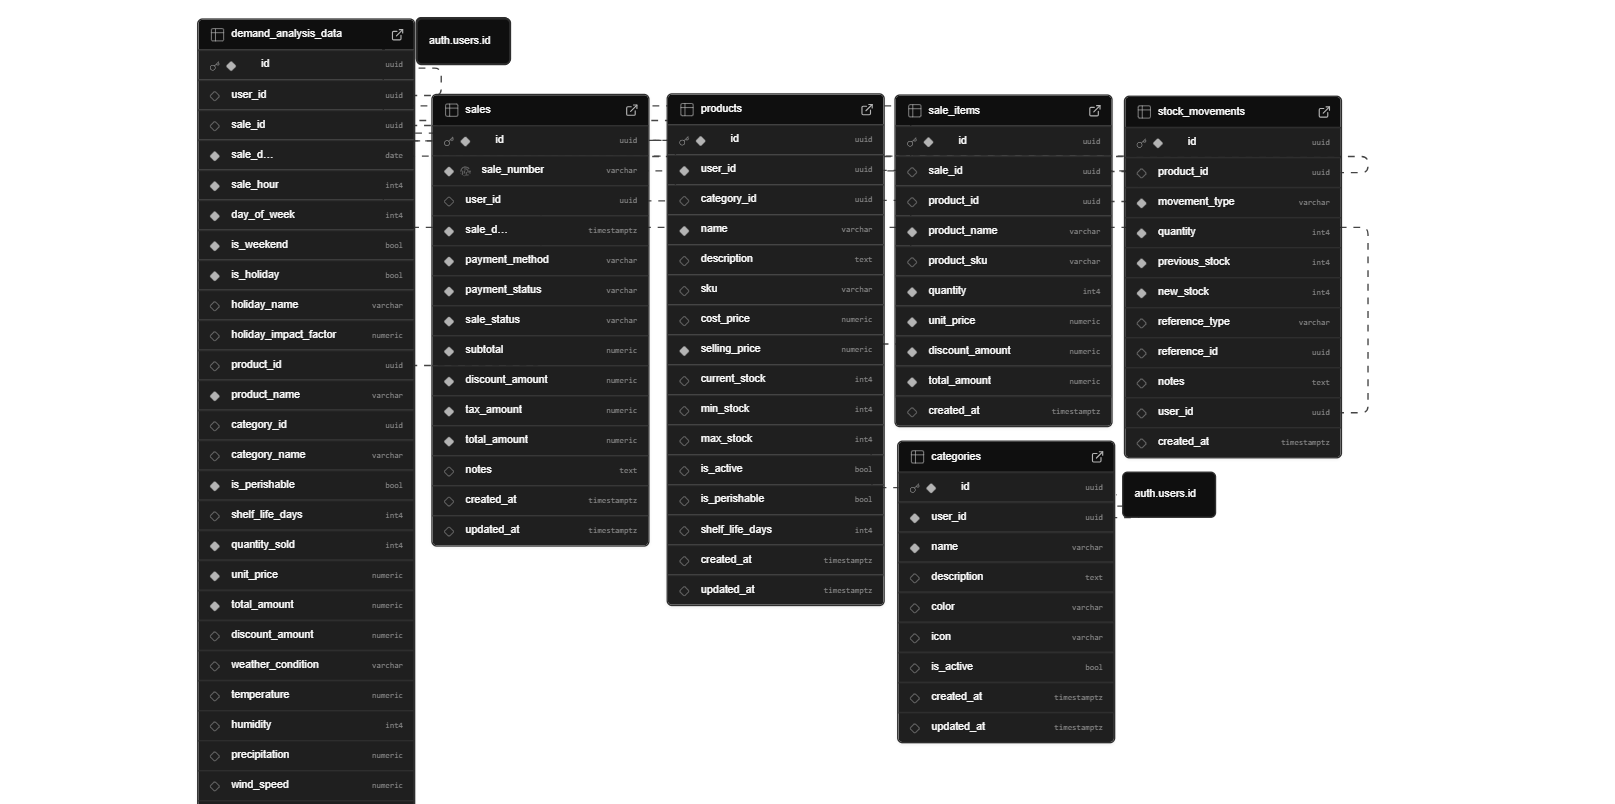
\includegraphics[width=0.95\textwidth]{images/ArquitecturaDB2.png} % <-- reemplazar por tu archivo
    \caption{Modelo de datos de AIVA 2-- Fuente: elaboración propia.}
    \label{fig:arquitectura-db2}
  \end{figure}
  \vspace{2cm}


\vspace{1cm}
\section{Diagrama de flujos}

Para describir el comportamiento dinámico del sistema incorporamos diagramas de flujo que muestran, paso a paso, cómo se procesan las operaciones clave. Estos esquemas complementan a los requerimientos y a la arquitectura estática, al hacer explícitas las secuencias, los puntos de decisión, los caminos alternativos y el manejo de errores, lo que facilita la validación funcional y el diseño de casos de prueba.


\subsection{DF-A · Autenticación}
El diagrama modela el control de acceso y el alta de usuarios. Se definió así para equilibrar seguridad (validaciones en el servicio de autenticación y verificación de correo), usabilidad (separación clara entre registro e inicio de sesión) y recuperabilidad (manejo de errores con retroalimentación inmediata). La convergencia final en el dashboard establece un único criterio de éxito y facilita la trazabilidad de estados; el objetivo es registrar las decisiones críticas del acceso sin describir pantallas intermedias.

\begin{figure}[!htbp]
  \centering
  \includegraphics[width=0.92\textwidth]{images/FlujoAutenticación.png}
  \caption{DF-A · Autenticación -- Fuente: elaboración propia}
  \label{fig:df-a-autenticacion}
\end{figure}


\subsection{DF-B · Carga de ventas}
El diagrama describe el proceso de registro de ventas desde dos orígenes complementarios: ingreso manual tipo POS y carga automática (OCR/CSV). Se define así para cubrir los escenarios operativos más frecuentes con validaciones progresivas y una confirmación explícita antes del alta, incorporando puntos de corrección para minimizar errores y preservar trazabilidad. La bifurcación temprana optimiza tiempos según la fuente de datos y el cierre en confirmación establece una única condición de éxito.

\begin{figure}[!htbp]
  \centering
  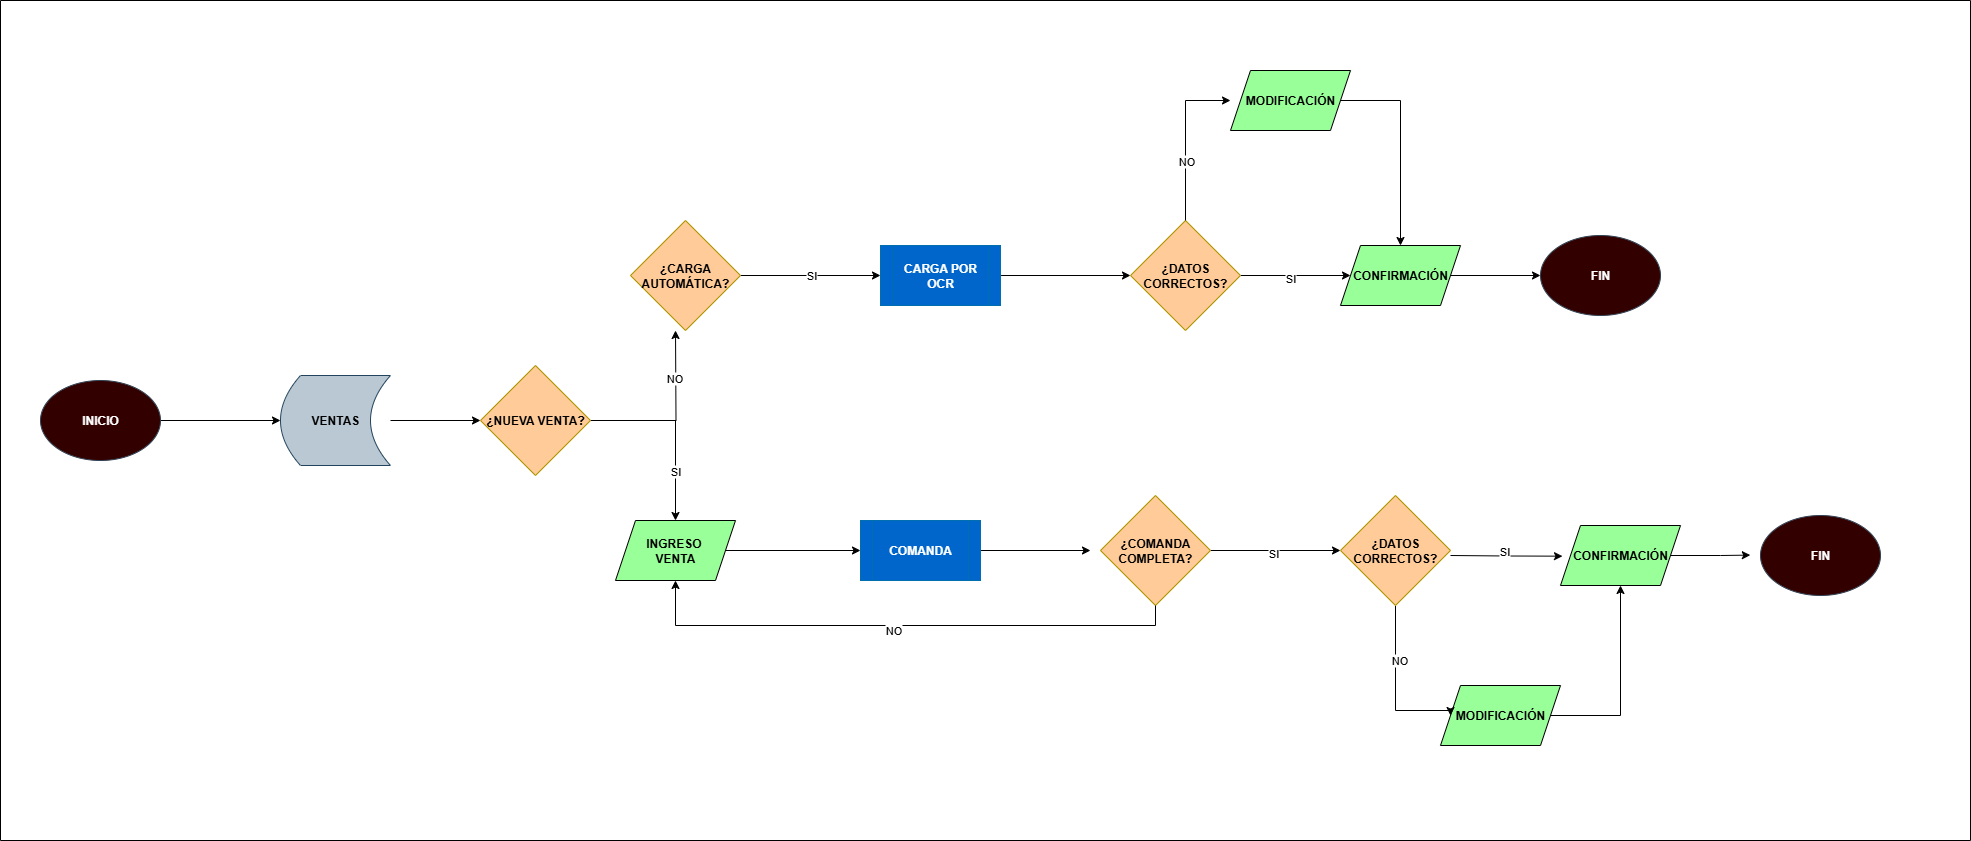
\includegraphics[width=0.92\textwidth]{images/FlujoVentas.drawio.png}
  \caption{DF-B · Carga de ventas -- Fuente: elaboración propia}
  \label{fig:df-b-ventas}
\end{figure}


\subsection{DF-C · Planes y suscripciones}
El diagrama describe la gestión de planes dentro de la aplicación. Al crear una cuenta, el usuario recibe automáticamente el plan gratuito; por este motivo, cualquier cambio de plan se realiza exclusivamente desde la app. El flujo contempla verificación de identidad y estado de suscripción, selección del nuevo plan y confirmación (incluida la validación de pago si corresponde). Ante éxito se actualiza la suscripción y se reflejan las capacidades en sesión; ante error se conserva el plan previo. El enfoque prioriza control de acceso, trazabilidad y una transición segura entre planes.

\begin{figure}[!htbp]
  \centering
  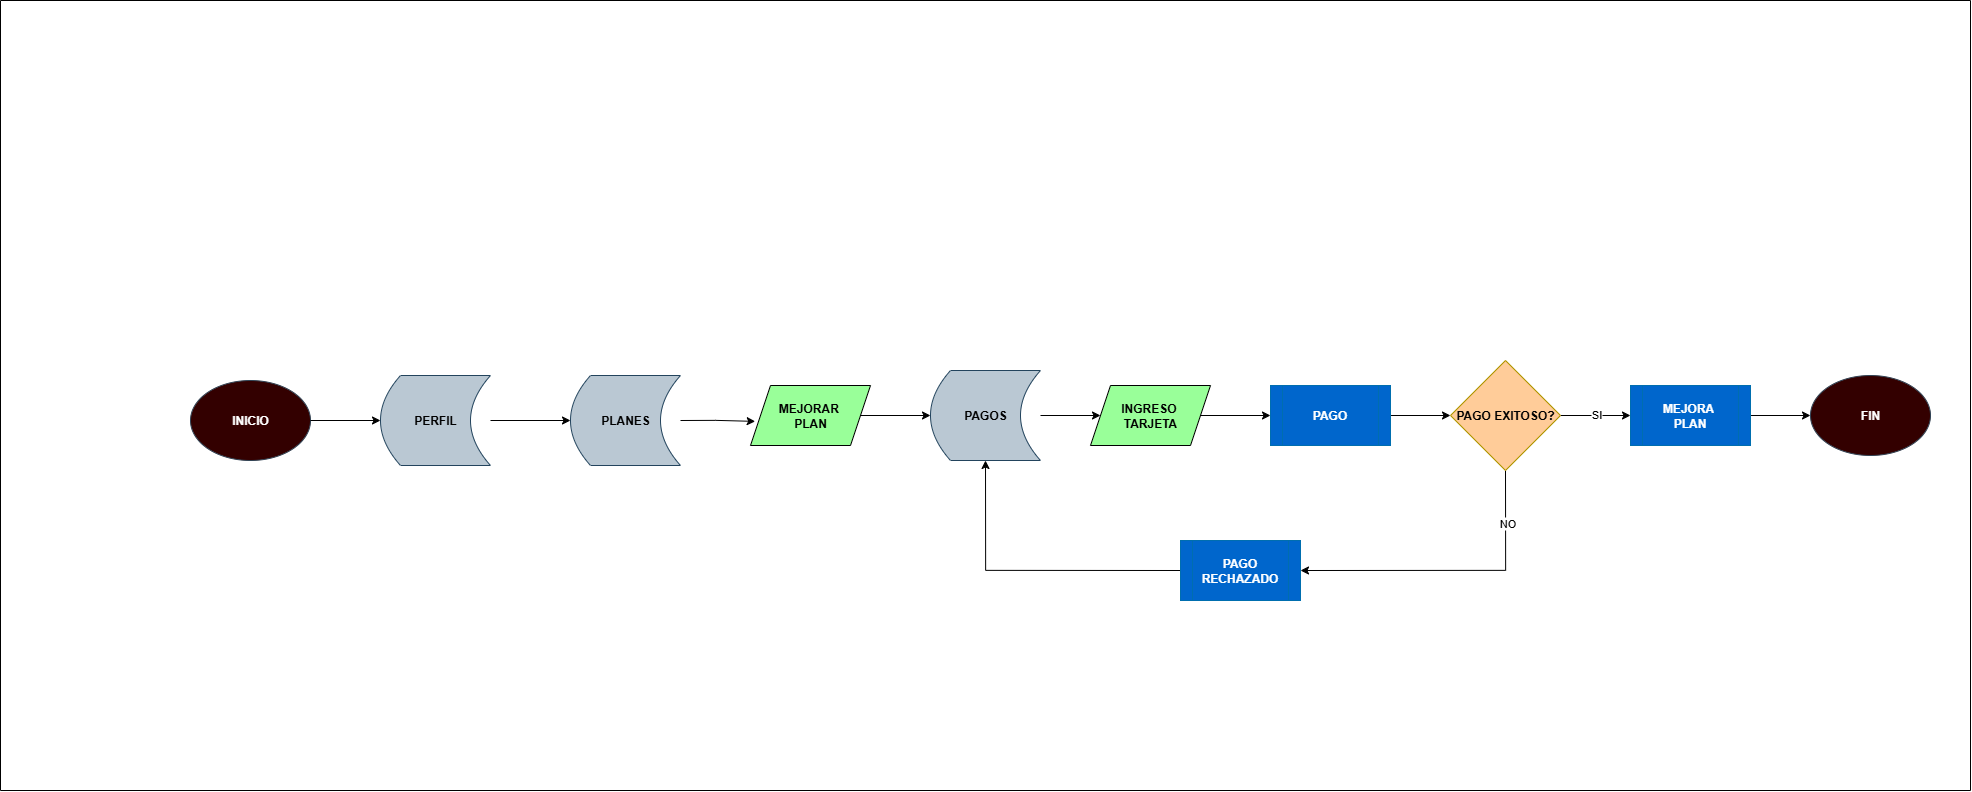
\includegraphics[width=0.92\textwidth]{images/FlujoPlanes.drawio.png}
  \caption{DF-C · Planes y suscripciones -- Fuente: elaboración propia}
  \label{fig:df-c-planes}
\end{figure}


\vspace{1cm}
\section{Identidad de marca}\label{sec:brand}

La identidad de marca de \textbf{AIVA} se diseñó para comunicar tecnología confiable, simplicidad operativa y foco en pequeños comercios. Esta sección documenta los elementos rectores de esa identidad y su relación con la experiencia de uso del sistema.

\subsection{Naming}
\textbf{AIVA} es un acrónimo de \textit{Asistente Inteligente para Ventas y Análisis}. El nombre cumple tres criterios: (i) \textit{memorabilidad} y pronunciación sencilla en español e inglés, (ii) \textit{brevedad} apta para interfaces y piezas breves (íconos, botones, navegación), y (iii) \textit{connotación} directa con analítica y apoyo a la decisión. El nombre se usa en mayúsculas para reforzar la legibilidad y la consistencia visual en la interfaz.

\subsection{Misión}
Poner la analítica predictiva al alcance de micro y pequeñas empresas de alimentos perecederos, reduciendo mermas y quiebres mediante planificación basada en datos. La misión orienta decisiones de producto hacia soluciones de bajo costo, fáciles de adoptar y con impacto operativo medible.

\subsection{Visión}
Constituirse en la plataforma de referencia en América Latina para la gestión de demanda en comercios de proximidad, integrando múltiples fuentes de datos (histórico, clima, calendario) y promoviendo prácticas sustentables de producción y reposición.

\subsection{Paleta de colores}\label{subsec:paleta}

La paleta cromática de \textbf{AIVA} fue definida para comunicar confianza tecnológica, claridad y foco en la toma de decisiones. El eje visual está compuesto por un rango de azules–índigo que se aplica en fondos y navegación, desde un índigo profundo hasta un azul más luminoso (\#1E2A78–\#3F6BFF). Esta base fría evoca precisión y estabilidad, atributos propios de una plataforma analítica, y refuerza la percepción de fiabilidad por parte del usuario.

Como acento de marca se incorpora el violeta (\#7C3AED, con su variante clara \#A78BFA), que introduce una connotación de innovación y modernidad. Este matiz se reserva para elementos de énfasis —botones primarios, indicadores destacados y piezas de comunicación—, logrando contraste visual sin perder coherencia con el tono profesional del sistema. Complementariamente, el cian (\#38BDF8) funciona como color informativo en enlaces y ayudas contextuales, guiando la atención sin distraer del contenido principal.

Los colores semánticos se emplean para codificar estados del sistema y facilitar la lectura operativa: el verde (\#22C55E) comunica confirmaciones y resultados positivos, mientras que el naranja (\#F59E0B) señala advertencias y situaciones que requieren seguimiento. La selección de saturación y brillo busca que estos mensajes sean perceptibles de forma inmediata, manteniendo, al mismo tiempo, una estética sobria adecuada al ámbito empresarial.

La familia de neutros se utiliza para garantizar legibilidad tipográfica y jerarquía en las superficies: un gris muy oscuro para textos (\#0F172A) y un gris claro para fondos (\#F1F5F9), complementados por blanco (\#FFFFFF) en componentes de alta claridad. En consonancia con pautas de accesibilidad, se privilegian combinaciones de alto contraste en las vistas más frecuentes, asegurando que la interfaz conserve nitidez tanto en entornos luminosos como en configuraciones de bajo brillo.

En conjunto, el gradiente principal de índigo a azul, el acento violeta y los semánticos verde/naranja construyen un lenguaje visual consistente: profesional en su base, expresivo en sus acentos y funcional en la comunicación de estados. Esta identidad cromática sostiene la experiencia de uso de AIVA y refuerza su posicionamiento como asistente inteligente para la gestión de demanda.

\begin{figure}[!htbp]
  \centering
  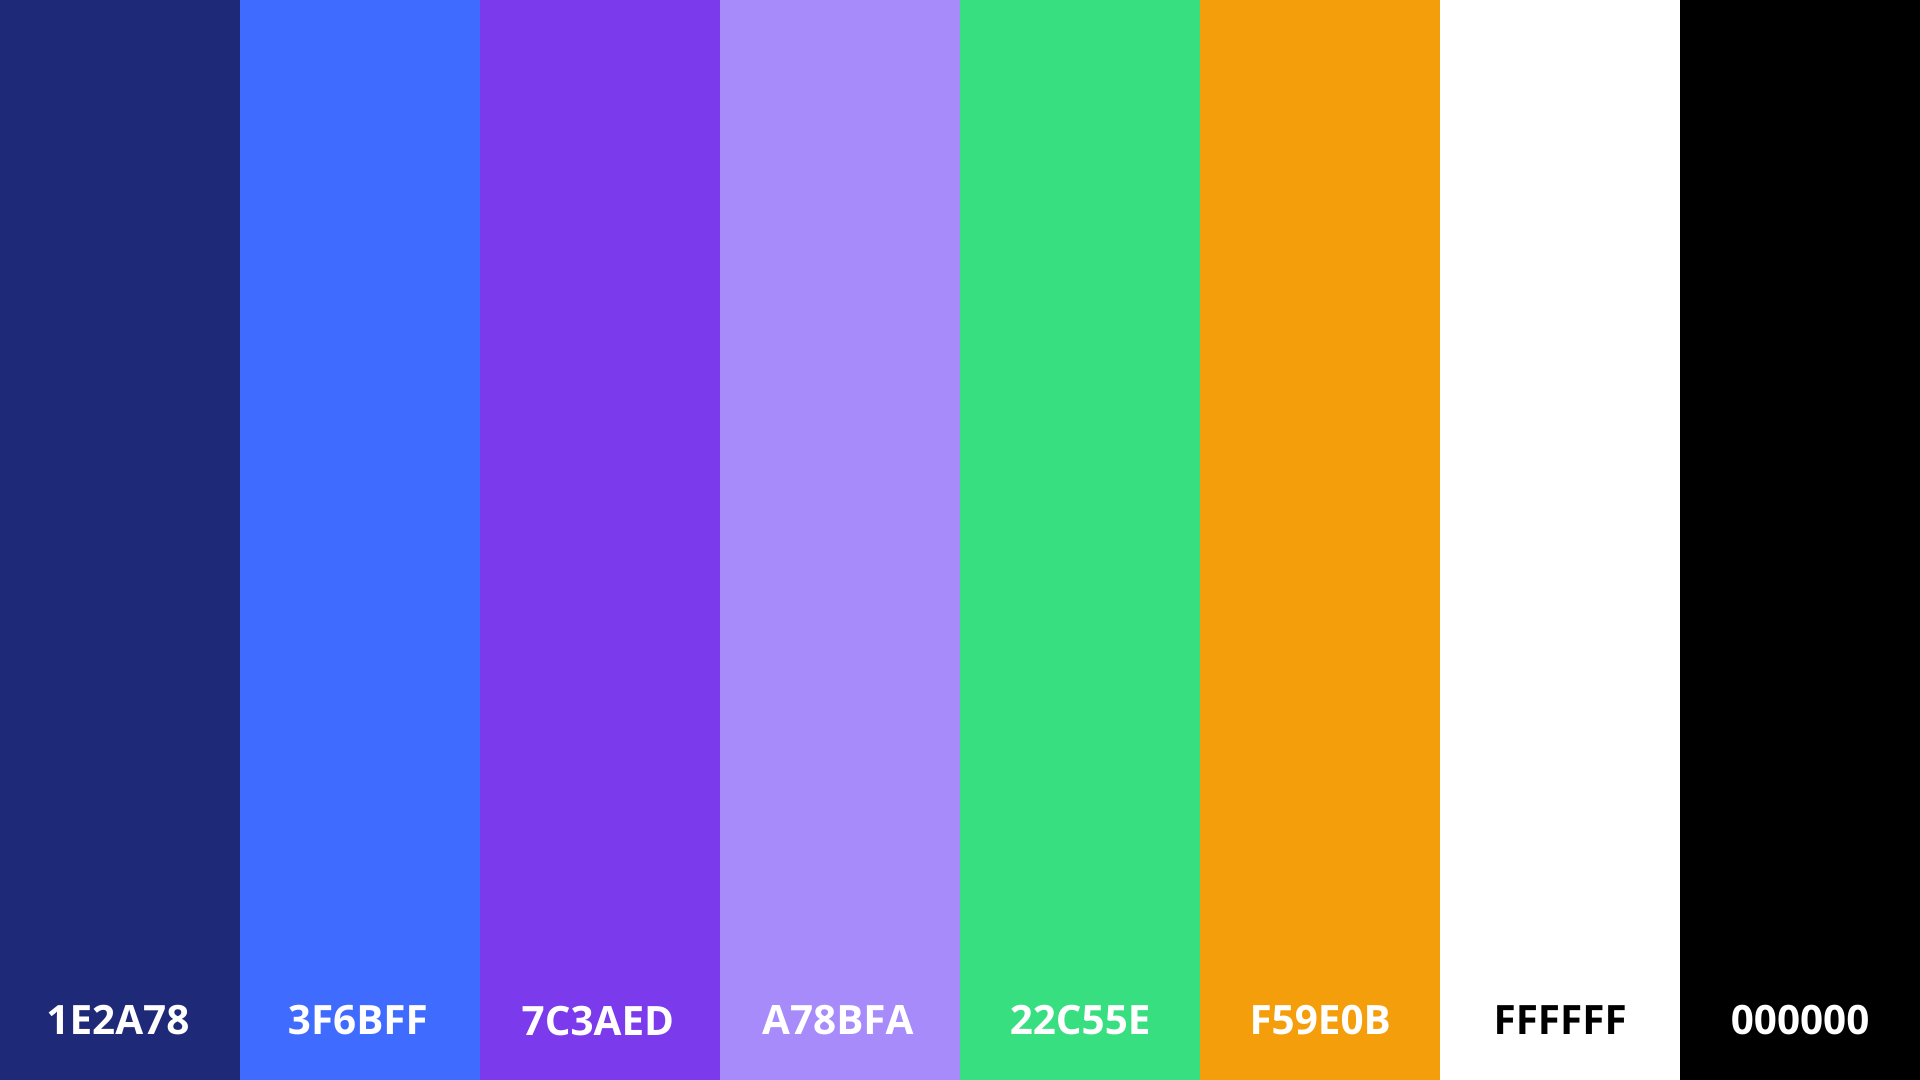
\includegraphics[width=0.92\textwidth]{images/paleta-aiva.png}
  \caption{Paleta de Colores -- Fuente: elaboración propia}
  \label{fig:paleta-aiva}
\end{figure}

\subsection{Logo}
El logotipo de AIVA representa la identidad visual del sistema y sintetiza su esencia conceptual y tecnológica. El nombre surge de la combinación de dos siglas: “AI”, correspondiente a Artificial Intelligence (Inteligencia Artificial), y “VA”, abreviatura de Valor Agregado. Esta fusión refleja la misión del proyecto de integrar inteligencia artificial aplicada a la predicción de demanda con un enfoque orientado a generar valor operativo, económico y ambiental para los pequeños comercios.

Desde el punto de vista visual, el logotipo está compuesto por un símbolo geométrico formado por cuatro módulos de distinta proporción que se agrupan en forma ascendente, evocando la idea de crecimiento, análisis y optimización de procesos. Este isotipo acompaña a la tipografía principal, moderna y de líneas rectas, que transmite precisión, confianza y solidez tecnológica.

La paleta cromática, en gradientes de azul, refuerza la noción de innovación y tecnología, mientras que el contraste con el texto blanco aporta claridad, legibilidad y profesionalismo. En conjunto, el diseño comunica los valores centrales de la marca: innovación, simplicidad y mejora continua mediante el uso de la inteligencia artificial.


\section{Metodología de desarrollo}\label{sec:metodologia}

El desarrollo del sistema se realizó siguiendo la metodología en cascada como modelo principal de ciclo de vida. Este enfoque, de naturaleza secuencial y estructurada, organiza el proceso de desarrollo en etapas claramente definidas: análisis, diseño, implementación, pruebas, despliegue y mantenimiento. La elección de esta metodología se basó en la necesidad de contar con una planificación detallada, documentación completa y un control riguroso del avance, condiciones adecuadas para proyectos con requerimientos bien delimitados y objetivos técnicos precisos.

En la fase de análisis, se relevaron los requerimientos funcionales y no funcionales del sistema, considerando tanto las necesidades de los usuarios finales como las restricciones técnicas. Posteriormente, durante el diseño, se elaboraron los diagramas de casos de uso, el modelo de datos y la arquitectura general de la aplicación, junto con las interfaces de usuario principales. En la etapa de implementación, se desarrollaron los módulos planificados conforme a las especificaciones definidas y siguiendo convenciones de codificación y documentación consistentes. Finalmente, las fases de pruebas y validación se centraron en verificar la correcta integración de los componentes, el desempeño general y la precisión de las predicciones generadas por el sistema.

Si bien la metodología en cascada fue la base del proceso, se introdujeron adaptaciones puntuales que permitieron incorporar instancias de retroalimentación sin alterar la estructura secuencial general. A lo largo del desarrollo se realizaron presentaciones intermedias del prototipo ante los tutores y revisores, con el propósito de obtener observaciones sobre la interfaz, la experiencia de uso y los resultados de predicción. Dichas revisiones posibilitaron efectuar ajustes menores en requerimientos y diseño, integrando comentarios relevantes sin modificar el orden de las fases principales. 

Esta adaptación otorgó flexibilidad al proceso, permitiendo mejorar la calidad del producto final y garantizar que las funcionalidades implementadas respondieran efectivamente a las necesidades validadas durante el seguimiento. En síntesis, el proyecto combinó la rigurosidad y trazabilidad del modelo en cascada con instancias controladas de retroalimentación iterativa, logrando un equilibrio entre planificación estructurada y capacidad de ajuste, adecuado para el desarrollo del sistema AIVA.


\vspace{1cm}

